\documentclass[12pt,a4paper]{article}
\usepackage[T1]{fontenc}
\usepackage[utf8]{inputenc}
\renewcommand{\familydefault}{\sfdefault}
\usepackage{graphicx}
\usepackage{verbatim}
\usepackage{float}
\usepackage{tikz}
\usepackage{pgfplots}
\usepackage{listings}
\pgfplotsset{compat=1.16}
\restylefloat{table}
\graphicspath{{Images/}}



\author{Vili Lipo, 014814253}
\title{Compilers Project 2020: Mini-pl interpreter documentation}
\begin{document}
\maketitle
\newpage

\section{General view of the application}
\subsection{Architecture}

\begin{figure}[t]\label{big_uml}
  \caption{UML diagram of the interpreter architecture}
  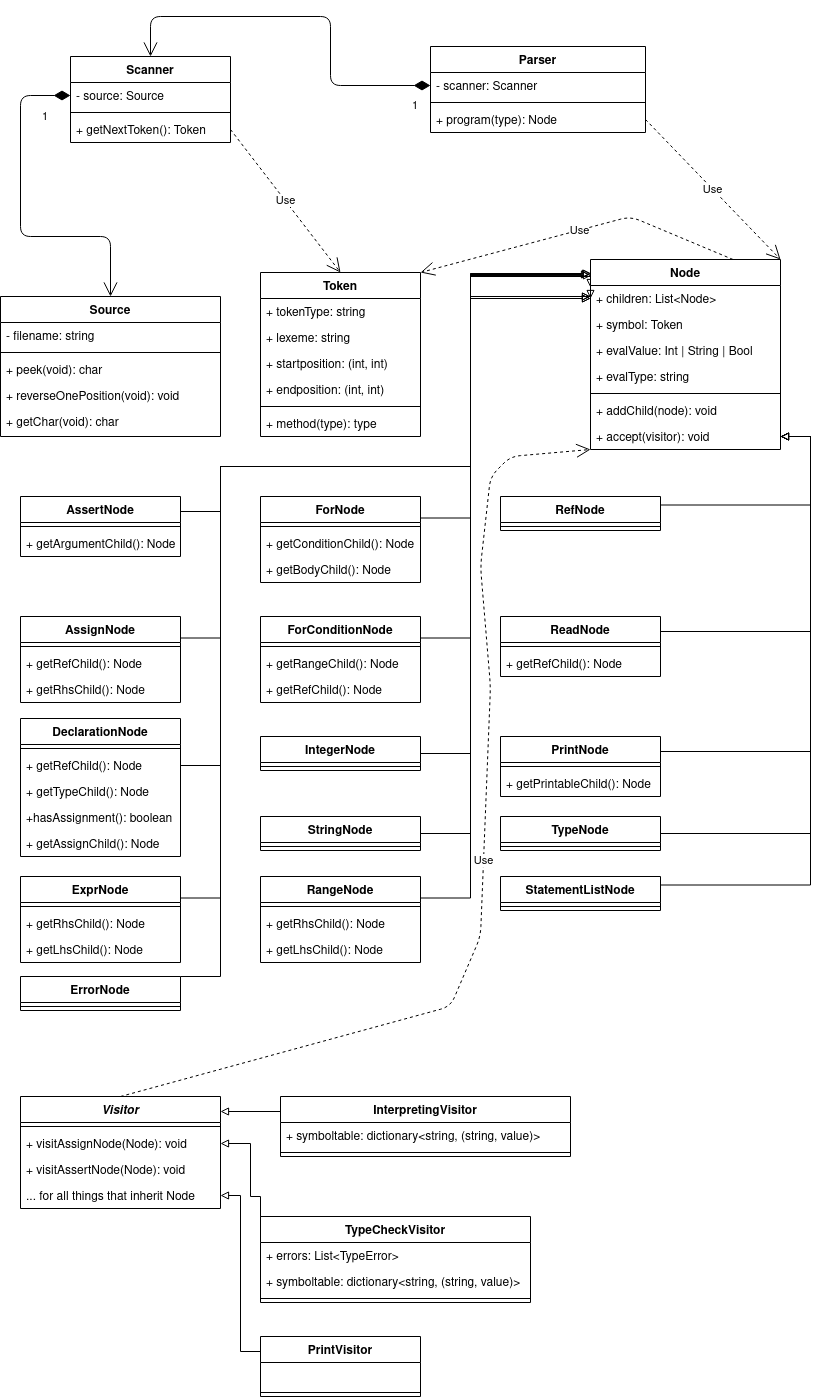
\includegraphics[scale=0.4]{reportImages/interpreter.png}
\end{figure}
The architecture of my implementation of Mini-pl interpreter
follows closely the pipeline pattern presented on the lectures.
The interpreter uses a multi-pass construction, as all of the
parsing is done before semantical analysis, and all semantical
analysis is done before the interpreting. The scanning
is driven by the parser, like in single pass compilers.

At the lowest level we have the class Source, that is responsible
for reading a source file and giving characters from it one by one.

This is given as a constructor parameter to the class Scanner following
the dependency injection pattern. Scanner
does the lexical analysis of the characters, and forms tokens out
of them. The Scanner consists of a collection of routines that
try to form a token by iterating the source. When a next
token is asked from the scanner it screens out whitespace and
comments and then it iterates through these
routines until one of them returns a valid token. If no
valid token is produced the scanner returns an error token.

When the source reaches the end-of-file the scanner produces
end of file token.

The parser is a recursive descent parser that asks for the tokens
one by one from the scanner. Every construct in the language has
a own method for parsing it. These methods produce abstract syntax 
tree nodes. The overall architecture can be observed in figure~\ref{big_uml}.

The abstract syntax tree produced by the parser
is first decorated by the TypeCheckVisitor, that
checks for semantical errors and creates a symbol table
based on variable declarations.

The table created by TypeCheckVisitor is then used by
InterpretingVisitor that interprets the source file.
InterpretingVisitor further decorates the abstract 
syntax tree by setting evaluation values to the nodes,
as it goes through the program.



\subsection{Testing}

The classes Source, Scanner and Parser have quite comprehensive
unit tests written to test their core functionality. Those
can be found in the '/tests' folder. I have taken care in 
designing these test cases and at least the tests for the
InterpretingVisitor and TypeCheckVisitor are worth to 
take look at.
Also the `tests/test.minipl' includes all the examples given
in the language specification.
The tests contain cases for producing correct error messages.

\begin{figure}\label{codecov}
  \caption{Unit and integration test code coverage}
  \begin{verbatim}
Name                                 Stmts   Miss  Cover
--------------------------------------------------------
interpreter/__init__.py                  0      0   100%
interpreter/ast.py                     179     13    93%
interpreter/interpretingvisitor.py     124      8    94%
interpreter/parser.py                  213     16    92%
interpreter/printvisitor.py             49      2    96%
interpreter/scanner.py                 153      3    98%
interpreter/source.py                   40      7    82%
interpreter/typecheckvisitor.py        157      5    97%
interpreter/visitor.py                  47     15    68%
tests/__init__.py                        0      0   100%
tests/testInterpretingVisitor.py        70      0   100%
tests/testParser.py                    160      0   100%
tests/testPrintVisitor.py               13      0   100%
tests/testScanner.py                   123      1    99%
tests/testSource.py                     23      1    96%
tests/testTypeCheckVisitor.py          131      1    99%
--------------------------------------------------------
TOTAL                                 1482     72    95%
  \end{verbatim}
\end{figure}

\subsection{Shortcomings}

The interpreter is mostly fully featured. 
The scanner supports only a limited set of escape characters that are
tabs, newlines, escape character and the quotation mark.
The parser is bit lacking
in the error handling part, as in most of the statements, if a 
necessary token is missing the parsing of that statement will fail,
and the exception handler will try to parse a new statement all together.

The Source class does not use any form of fancy buffering. It just reads
the whole file to a list of strings in its constructor. I did not think
that any buffering of source was justified as most of the programs 
that would be written using Mini-pl are short. Even in very powerful
languages most code style guides prefer files under five hundred lines with
a line length under 100 characters. Any modern computer is able to hold
5000 characters in its memory with no issues.

\subsection{Running the program}

On Linux-machines running this program should be very straight forward.
Open the directory where the archive was unzipped in a terminal.
Then running 
`python3 main.py ./tests/test.minipl'
There is no additional external dependencies in runnign the program,
everything should be included in the python standard library.


\section{Specifying the interpretation}

\subsection{Mini-PL token patterns}
The token patterns can be observed in figure~\ref{token_patterns}
\begin{figure}\label{token_patterns}
  \caption{Mini-PL token patterns}
  \begin{verbatim}
  <integer> ::= <digit>*
  <string_literal> = "<alnum>*"
  <identifier> = ([a-z] | [A-Z])([a-z] | [A-Z] | _ | [0-9])*
  <range> ::= \.\.
  <keyword> ::= var | for | end | in | do | read 
  <keyword> ::=  print | int | string | bool | assert
  <operator> ::= + | - | / | * | & | !
  \end{verbatim}
\end{figure}

\subsection{Context-free grammar}
The modified context-free grammar for Mini-pl can be seen in figure~\ref{cfg}
\begin{figure}\label{cfg}
  \caption{Modified LL (1) grammar for Mini-pl}
  \begin{verbatim}
  <prog> ::= <stmnts>
  <stmts> ::= <stmnt> ";" <stmnts>
  <stmnts> ::= <epsilon>
  <stmnt> ::= "var" <identifier> : <type> <assign_value>
  <stmnt> ::= <identifier> ":=" <expr>
  <stmnt> ::= "for" <identifier> "in" <expr> .. <expr> "do" <stmnts> end for
  <stmnt> ::= "read" <identifier> 
  <stmnt> ::=  "print" <expr>
  <stmnt> ::= "assert" ( <expr> )
  <assign_value> = := <expr>| <epsilon>
  <expr> ::= <opnd> <op> <opnd>
  <expr> ::= <unary_op> <opnd>
  <opnd> ::= <integer>
  <opnd> ::= <string_literal>
  <opnd> ::= <identifier>
  <opnd> ::= ( <expr> )
  <type> ::= "int"
  <type> ::= "string"
  <type> ::= "bool"

  \end{verbatim}
\end{figure}

\subsection{Abstract syntax tree}
The abstract syntax tree used in the interpreter, uses the composite pattern and visitor
pattern is used to manipulate the tree. The base class Node and its descendants are
defined in the file `./interpreter/ast.py'

\subsection{Error Handling}

When the scanner encounters an error it sends an error token to the parser.

The parser uses context sensitive lookahead with exception driven error
handling to recover from syntax errors. Because of the way how the error
handling is written statements that are not able to be parsed will not show up
in the AST built by the parser, as the statement routine sees that there is
another symbol next, that is in its first set.

Semantic errors are discovered by TypeCheckVisitor.
These errors are printed to the user and prevent the interpreting process.

\subsection{Semantics of Mini-pl}

I have adjusted the semantics of Mini-pl a bit. In the specification
it seems that the loop variable should be one over the upper limit of the 
specified range. In my implementation when the loop ends, the loop variable
is the upper limit of the range. In essence my range is a open interval.

As for variable default values I have chosen 0 for integer, empty string for string, and 
false for boolean.

\section{Work hour log}



\end{document}
